\chapter*{MAC OS}

\section*{INICIOS DE MACINTOSH OPERATING SYSTEM}
Más conocido como MAC OS tuvo sus inicios en el año 1984 con
el sistema 1.0 que era a blanco y negro, con una pantalla
pequeña. inicialmente el sistema operativo mac era instalado en
equipos con el diseño de un todo en uno como los de hoy en día
con una pantalla de 9 pulgadas y su resolución de 520 x 342.
necesitaba 192KB para su instalacion y fue uno de los primeros
sistemas operativo en implementar la interfaz del usuario, con la
fortuna de haber sido el más exitoso ya que a diferencia de otros
sistemas operativos era muy amigable y de facil uso para el
usuario.

Algo muy peculiar es que no habia jerarquías de carpetas ya que
solo existía una donde se alojaban todos los archivos algo
bastante molesto al momento de buscar algún archivo; a
diferencia de otros sistemas operativos system 1.0 contaba con
un explorador de archivos propio llamado finder que tenia que
tenia cuatro menús en la parte superior muy similares a los de
hoy en dia.

\subsection*{PANEL DE CONTROL}

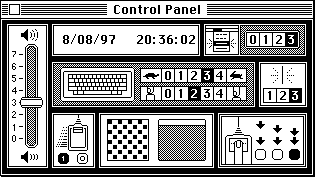
\includegraphics[scale=0.5]{img/cp09/img0901.png}

Definitivamente el
panel de control si los
va a sorprender, era
bastante intuitivo y
con funciones muy
peculiares, a la
izquierda vemos el
nivel de volumen, en
la parte superior
estaba la fecha y hora,
el siguiente era para
configurar cuantas
veces parpadea el menú al momento de seleccionarlo,
el menú del centro era un poco confuso ya que es para las
repeticiones de las teclas y una velocidad de retraso, el
siguiente es la velocidad del cursor al momento estar en un
programa de edición de texto, ya en la parte inferior del panel
encontramos la velocidad del mouse, el siguiente es para el
fondo de pantalla usted dibujaba un patrón a la izquierda y al
momento que le daba click en el cuadro de la derecha ya
quedaba dibujado en el escritorio y para terminar era ya era
para controlar la velocidad del doble click.

Tuve la experiencia de manejar el sistema operativo system
software 7.0.1 gracias a un emulador llamado mini vmac y la
experiencia como usuario fue bastante agradable ya que el
manejo fue muy similar al sistema operativo de hoy dia con la
diferencia que al momento de ingresar al menu tenia que tener
sostenido el click e ir bajando con el cursor y para seleccionarlo
soltar el click, algo muy incomodo, pero en general fue un
sistema muy amigable y para las personas de la época creería
que era un sistema operativo bastante innovador y llamativo.

adaptado de http://www3.nd.edu/~jvanderk/sysone/

\section*{HOY EN DÍA MAC OS X MAVERICKS}

A grandes rasgos mac os mavericks es la última versión del
sistema operativo mac esta especialmente hecha para todas las
computadoras de la marca apple, esta basado en UNIX, y es
considerado uno de los mejores sistemas operativos del mundo
hablaré del diseño, la seguridad, pero más que todo me enfocaré
en su alto rendimiento ya que sin duda esta es la característica
más importante para mi y la mayoría de las personas que
laboran en la industria de la música y el diseño gráfico.

\subsection*{DISEÑO}

Tiene una interfaz gráfica muy amigable con el usuario y
realmente se esforzaron en que tuviera un aspecto brillante,
algo que la caracteriza es su estilo que da una apariencia
sofisticada y elegante ya que tuvieron en cuenta cada detalle
para que se mirara como lo es.

\subsection*{MENUS}

Este sistema operativo cuenta con un menú en la parte superior
de la pantalla que se adapta a la aplicacion que tenga abierta,
para las opciones de (archivo, editar, ver, ventana, ayuda) cabe
aclarar que depende la aplicacion asi mismo tendra sus
variaciones. También cuenta con una barra de accesos directos
de aplicaciones, carpetas y archivos llamado “dock” en la parte
inferior de la pantalla, este dock ayuda a que nuestro escritorio
está siempre vacío ya que por defecto lo que allá en el escritorio
se podria decir que esta abierto, esto es algo diferente a los
demás ya que así cerremos la aplicacion con la “X” localizada en
la parte superior izquierda, las aplicaciones siguen abiertas en
un segundo plano, Realmente para poder cerrar las aplicaciones se puede dar click
derecho o click con 2 dedos con el trackpad encima del icono del
dock ahy le saldra una opcion de salir, hasta ese momento
realmente se habrá cerrado la aplicacion o para poder cerrarlo
más de una forma menos engorrosa con el atajo del teclado que
seria la tecla (command + q ).

\subsection*{LAUNCHPAD Y MISION CONTROL}

Una alternativa al dock es el launchpad, se trata de una
aplicacion donde muestra todas las aplicaciones que tiene el
equipo y las muestra en forma de cuadrícula donde se pueden
agrupar y crear subcarpetas o de forma individual como viene
por defecto es una forma muy creativa de mostrarnos cuales son
los programas instalados en nuestro equipo.

Otra herramienta que tenemos es el mission control que nos
permite ver que aplicaciones tenemos abiertas, recordando que
también tenemos aplicaciones corriendo en segundo plano nos
permite tener múltiples escritorios abiertos, algo realmente
necesario para los usuarios que necesitan hacer varias cosas a la
vez sin estar minimizando las ventanas. dentro del mission
control encontramos también aplicaciones básicas como
(calculadora, hora mundial, tiempo, notas, traductor) entre otras
que ud puede descargar.

\subsection*{SEGURIDAD}

Otro aspecto que diría que es muy importante es que es libre de
virus, el usuario tiene la seguridad que no tendrá que reinstalar
sus sistema operativo porque un virus daño su sistema de
arranque o algo muy conocido entre los usuarios de windows es
que las carpetas quedan ocultas y solo puedes ver los accesos
directos, con este sistema operativo estos eventos muy poco
productivos quedarán en el olvido.

\section*{PRODUCCIÓN MUSICAL}

En la producción musical los computadores mac ha tenido un
impacto grandísimo ya que son los preferidos en los estudios
musicales no solo por su diseño si no tambien por que brindan
una estabilidad y confiabilidad de que no va a tener errores
inesperados, esto quiere decir que ni se va a detener el
programa ni se va a cerrar.

\subsection*{GARAGE BAND}

Empezaré hablando de Garage Band es un programa que ya
viene instalado en el sistema operativo, aunque al principio
costó creer que fuera gratis porque el programa es bastante
completo en el tema de la producción musical ya que puedes
desde grabar, mezclar, producir y masterizar un tema musical
todo con este programa y esta especialmente hecho para mac
que le da más estabilidad.

Garabe Band tiene una característica muy importante, nos
permite utilizar VST o Virtual Studio Technology (Tecnología
de Estudio Virtual) es una interfaz estándar desarrollada por
Steinberg para conectar sintetizadores de audio y plugins de
efectos a editores de audio y sistemas de grabación. Permite
reemplazar el hardware tradicional de grabación por un estudio
virtual con herramientas software.

En otras palabras lo que hace un VST es simular un instrumento
musical(piano,guitarra,violin,sintetizador,etc) para que la gente
no tenga que comprarse un instrumento real,o por que un
instrumento ya no existe pero si existe su vst que simula el 99\%.

Un VST es un programa de software que debe ser ejecutado
mediante una aplicación que soporte esta tecnología. A esta
aplicación se le llama VST Host, ejemplos de esto son Cubase,
FL Studio, Ableton Live, entre otros.
También existen los VSTI (Virtual Studio Technology
Instruments) que es tocar mediante interfaces que utilizan el
protocolo midi, esto le permite al usuario hacer canciones sin
tener que comprar ningún instrumento que es una ventaja para
las personas que quieren hacer algo muy parecido a lo real de
una forma virtual sin tener conocimiento avanzados en tocar un
instrumento y reduciendo costo de manera muy significativa.
También da la opción de trabajar usando interfaces de sonido
que permitan la captura del sonido de un instrumento real o la
voz de una persona para su posterior mezcla, produccion, post
produccion y remasterizacion.tambien para los usuarios novatos
dentro del mismo programa existen tutoriales para hacer una
canción haciendo solo click y seleccionando loops o pistas cortas
ya estableciodas y juntandolos, solo es tener un buen oido y
ganas de aprender.

\subsection*{PROTOOLS}

Pro Tools es una estación de trabajo de audio digital (Digital
Audio Workstation o DAW, en inglés), una plataforma de
grabación, edición y mezcla multipista de audio y midi, que
integra hardware y software. Por sus altas prestaciones, es el
considerado el estándar de grabación, edición y mezcla en
estudios profesionales y postproducción, usado mundialmente.

Pro Tools inicia en 1989 llamándose "sound tools" para
plataforma Apple Macintosh, la compañía se refiere a este como
el primer estudio de grabación "Tapeless" (Sin cinta). Solo
grababa 2 pistas con calidad de CD y funcionaba en un
computador Macintosh.En 1994 Digidesign lanza Pro-Tools III
que se establece como líder absoluto y convirtiéndose en el
sistema más poderoso creado hasta la fecha de un sistema de
grabación de sonido a disco duro.

En 1991 aparece el primer sistema "multi-track", marcando un
gran avance en el audio digital y que rápidamente se transforma
en la más popular estación de trabajo para producción de TV,
música y películas por su integrado diseño entre el software y
hardware. Este podía grabar de 16 a 42 pistas y era posible
conectar de 8 a 64 canales físicos, según el tipo de interface.
Además, poseía un mezclador y procesaba el audio mediante
aplicaciones llamadas Plug-Ins, en los cuales encontramos:
compresores y efectos como delays, limitadores, vocoders,
emuladores de sintetizadores clásicos, samplers virtuales, etc.

Para que funcione correctamente Pro-Tools III, se necesitaba un
computador Macintosh con una ranura llamada "NuBus", la que
al cabo de unos años se transformó en los puertos PCI, SCSI, y
ahora último USB y Firewire. Así Pro-Tools III, en su sistema
más sencillo era el Software en sí y además la tarjeta llamada
Disk I/O, la cual era insertada en el computador y se conectaba a
su vez a la interface de audio, que era la que permitía conectar
las entradas y salidas de audio para poder grabar y monitorear.

Estas Interfaces de Audio eran las 888 y 882 de Digidesign y sus
diferencias eran básicamente sus tipos de conectores, la primera
poseía 8 entradas y salidas con conectores balanceados XLR o
Canon, mientras que la 882 poseía 8 entradas y 8 salidas
balanceadas con conectores 1/4 plug.

Los requerimientos del computador para que funcionase ProTools
III, eran: Computador Macintosh, con Interfase o ranura
Nubus o PCI, procesador de 120 Mhz, Memoria Ram mínimo de
16 MB, Sistema Operativo 7.1 o superior, un Monitor, y además
era recomendable un disco duro externo.


